\section{Comunicação serial}

RS-232 é uma comunicação full-duplex(ida e volta ao mesmo tempo). Os sinais são
representados com voltagens em relação ao ground(chamado common). Ele possui 
muitas linhas de handshaking. O sinal muitas vezes está entre -12V e +12V,
sendo -3V e +3V usados para absorver ruídos.

Os sinais na Cyclone para comunicação serial são \verb|UART_TXD| para envio e
\verb|UART_RXD| para receber. O protocolo de comunicação é ilustrado na 
figura~\ref{simulacao}. Cada pacote possui 10 bits, 8 bits de dado e dois para
start e stop. Além disso é necessário um prescaler no código que implementa esse
protocolo, ele deve contar de 0 até 5208, já que 50MHz/9600 Bit/sec = 5208. 9600
é o baud rate da serial. Assim sabemos o tempo que se deve aguardar na contagem,
usando o clock, para igualar o baud rate. Esse método é muito usado em FPGAs
para fazer o timing com unidades externas, como memória RAM, etc.

\begin{figure}[!h]
\centering
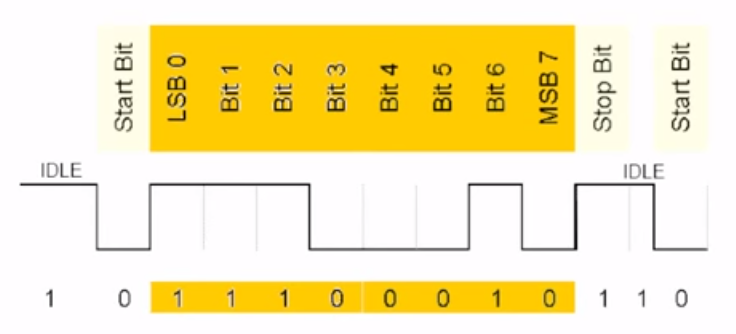
\includegraphics[width=3.3in]{img/uart.png}
% where an .eps filename suffix will be assumed under latex, 
% and a .pdf suffix will be assumed for pdflatex; or what has been declared
% via \DeclareGraphicsExtensions.
\caption{Esquema de transmissão serial.}
\label{simulacao}
\end{figure}